\begin{document}

\def\title{Worksheet 10}

\newcommand{\qitem}{\qpart\item}

\renewcommand{\labelenumi}{(\alph{enumi})} % change default enum format to (a)
\renewcommand{\theenumi}{(\alph{enumi})} % fix reference format accordingly.
\renewcommand{\labelenumii}{\roman{enumii}.} % second level labels.
\renewcommand{\theenumii}{\roman{enumii}.}
\renewcommand{\arraystretch}{1.25}

\maketitle

\vspace{0.5em}

\begin{qunlist}
    \qns{Graph Linearization}
\qcontributor{Sirej Dua}
 
 I linearized a function, and printed a graph of what the linearization, but then I carelessly I lost the original function. This is a plot of the linearization.

    Which of the following functions, linearized about $x=0$, could have been my function? \\

    1. $3x + \cos x - 1$, \\
	2. $3x$,\\
	3. $x + 2e^x - 2$,\\

    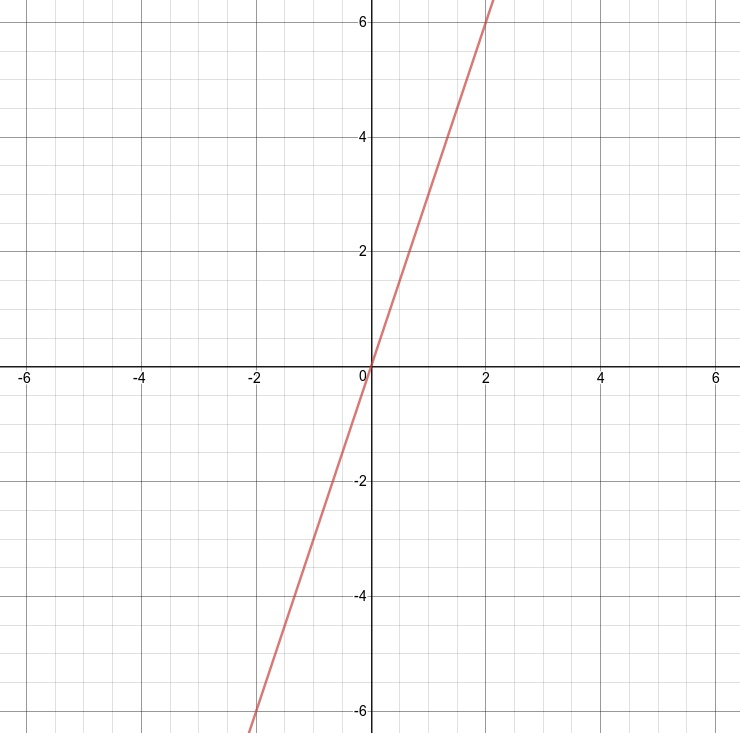
\includegraphics[scale=0.4]{\bank/linearization/figures/line.png}

    
	\sol{
	All three can be linerized about $x=0$ to the function in the graph.



	% TODO: detailed explanation
	}

    % Author: Naomi Sagan
% Emails: naomi.sagan@berkeley.edu

\qns{Jacobian Intuition}

In this problem, we will build the intuition behind constructing the Jacobian matrix used for linearizing systems of nonlinear functions. \\
\newline
For this problem, consider the following system of functions in terms of $\vec{x} = \begin{bmatrix} x_1 \\ x_2 \end{bmatrix}$:
\begin{align*}
    f_1(x_1, x_2) = x_1^3 + \sin(x_2) \\
    f_2(x_1, x_2) = e^{2x_1} - x_2 - 1
\end{align*}
Let the operating point about which you linearize the system be
\begin{align*}
    \vec{x}^{*} = \begin{bmatrix} 0 \\ 0 \end{bmatrix}
\end{align*}

\begin{enumerate}
    \qitem Find the linear approximation of $f_1$ about $\vec{x}^{*}$.
    \begin{align*}
        f_1(x_1, x_2) \approx f_1(x_1^{*}, x_2^{*}) + \frac{\partial f_1}{\partial x_1} \bigg\rvert_{\vec{x*}} (x_1 - x_1^{*}) + \frac{\partial f_1}{\partial x_2} \bigg\rvert_{\vec{x*}} (x_2 - x_2^{*})
    \end{align*}
    \begin{enumerate}[label = (\roman*)]
        \item First, take $x_2$ as constant. What is the linear approximation of $f_1(x_1, x_2^{*})$? \\
        \sol{
            If we take $x_2$ as constant, the approximation of $f_1$ is as follows:
            \begin{align*}
                f_1(x_1, x_2^{*}) \approx f_1(x_1^{*}, x_2^{*}) + \frac{\partial f_1}{\partial x_1} \bigg\rvert_{\vec{x*}} (x_1 - x_1^{*})
            \end{align*}
            Notice that $f_1(\vec{x}^{*}) = 0$, so 
            \begin{align*}
                f_1(x_1, x_2^{*}) \approx \frac{\partial f_1}{\partial x_1} \bigg\rvert_{\vec{x*}} (x_1 - x_1^{*})
            \end{align*}
            Taking the partial derivative of $f_1$ with respect to $x_1$:
            \begin{align*}
                f_1(x_1, x_2^{*}) \approx 3(x_1^{*})^2(x_1 - x_1^{*})
            \end{align*}
            Plugging in $x_1^{*} = 0$, we get
            \begin{align*}
                f_1(x_1, x_2^{*}) \approx 0
            \end{align*}
        }
        \item Now, take $x_1$ as constant. What is the linear approximation of $f_1(x_1^{*}, x_2)$? \\
        \sol{
            If we take $x_1$ as constant, the approximation of $f_1$ is as follows:
            \begin{align*}
                f_1(x_1^{*}, x_2) \approx f_1(x_1^{*}, x_2^{*}) + \frac{\partial f_1}{\partial x_2} \bigg\rvert_{\vec{x*}} (x_2 - x_2^{*})
            \end{align*}
            Plugging in $\vec{0}$ for $\vec{x}^{*}$:
            \begin{align*}
                f_1(x_1^{*}, x_2) \approx \frac{\partial f_1}{\partial x_2} \bigg\rvert_{\vec{0}} \cdot x_2
            \end{align*}
            Taking the partial derivative of $f_1$ with respect to $x_2$:
            \begin{align*}
                f_1(x_1^{*}, x_2) \approx \cos(x_2^{*}) \cdot x_2 = x_2
            \end{align*}
        }
        \item Now, what is $f_1(x_1, x_2)$ linearized around $\vec{x}$? \\
        \sol{
            To find the linear approximation of $f_1$ with respect to both $x_1$ and $x_2$, add the approximation of $f_1$ that depends on $\frac{\partial f_1}{\partial x_1}$ to the approximation that depends on $\frac{\partial f_1}{\partial x_2}$.
            \begin{align*}
                f_1(x_1, x_2) \approx f_1(x_1^{*}, x_2^{*}) + \frac{\partial f_1}{\partial x_1} \bigg\rvert_{\vec{x*}} (x_1 - x_1^{*}) + \frac{\partial f_1}{\partial x_2} \bigg\rvert_{\vec{x*}} (x_2 - x_2^{*})
            \end{align*}
            Remembering that $f_1(x_1^{*}, x_2^{*}) = 0$ and plugging in the results from parts (i) and (ii), we have
            \begin{align*}
                f_1(x_1, x_2) \approx 0 + 0(x_1) + x_2 = x_2
            \end{align*}
        }
    \end{enumerate}

    \qitem Using the same process as in part (a), find the linear approximation of $f_2$ about $\vec{x}^{*}$. \\
    \sol {
        First, find the partial derivative of $f_2$ with respect to $x_1$, evaluated at the operating point $\vec{x} = \vec{0}$:
        \begin{align*}
            \frac{\partial f_2}{\partial x_1} \bigg\rvert_{\vec{x*}} = 2e^{2x_1^{*}} = 2e^0 = 2
        \end{align*}
        Then, find the partial derivative of $f_2$ with respect to $x_2$ at the operating point:
        \begin{align*}
            \frac{\partial f_2}{\partial x_2} \bigg\rvert_{\vec{x*}} = -1
        \end{align*}
        Then, the linear approximation of $f_2$ is:
        \begin{align*}
            f_2(x_1, x_2) \approx f_2(x_1^{*}, x_2^{*}) + \frac{\partial f_2}{\partial x_1} \bigg\rvert_{\vec{x*}} (x_1 - x_1^{*}) + \frac{\partial f_2}{\partial x_2} \bigg\rvert_{\vec{x*}} (x_2 - x_2^{*}) \\
            f_2(x_1, x_2) \approx 0 + 2(x_1 - 0) - 1(x_2 - 0) = 2x_1 - x_2
        \end{align*}
    }

    \qitem Now, we want to approximate $\vec{f}(\vec{x}) = \begin{bmatrix} f_1(\vec{x}) \\ f_2(\vec{x}) \end{bmatrix}$ around $\vec{x} = \vec{0}$ as a matrix-vector equation.
    \begin{align*}
        \vec{f}(\vec{x}) \approx \vec{f}{\vec{x}^{*}} + J_{\vec{x}}(\vec{x} - \vec{x}^{*})
    \end{align*}
    Fill in the Jacobian, $J_{\vec{x}}$, by finding the constants $a, b, c, d$ that complete the following equation:
    \begin{align*}
        \begin{bmatrix}
            f_1(\vec{x}) \\
            f_2(\vec{x})
        \end{bmatrix} \approx
        \begin{bmatrix}
            f_1(\vec{x}^{*}) \\
            f_2(\vec{x}^{*})
        \end{bmatrix} +
        \begin{bmatrix}
            a & b \\
            c & d
        \end{bmatrix} 
        \begin{bmatrix}
            x_1 - x_1^{*} \\
            x_2 - x_2^{*}
        \end{bmatrix}
    \end{align*}

    \sol{
        $a$ is the component of the approximation of $f_1$ that multiplies $x_1$:
        \begin{align*}
            a = \frac{\partial f_1}{\partial x_1} \bigg\rvert_{\vec{x*}} = 0
        \end{align*}
        $b$ is the component of the approximation of $f_1$ that multiplies $x_2$:
        \begin{align*}
            b = \frac{\partial f_1}{\partial x_2} \bigg\rvert_{\vec{x*}} = 1
        \end{align*}
        $c$ is the component of the approximation of $f_2$ that multiplies $x_1$:
        \begin{align*}
            c = \frac{\partial f_2}{\partial x_1} \bigg\rvert_{\vec{x*}} = 2
        \end{align*}
        $d$ is the component of the approximation of $f_2$ that multiplies $x_2$:
        \begin{align*}
            d = \frac{\partial f_2}{\partial x_2} \bigg\rvert_{\vec{x*}} = -1
        \end{align*}

        So, the linear approximation of the system is as follows:
        \begin{align*}
        \begin{bmatrix}
            f_1(\vec{x}) \\
            f_2(\vec{x})
        \end{bmatrix} \approx
        \begin{bmatrix}
            f_1(\vec{0}) \\
            f_2(\vec{0})
        \end{bmatrix} +
        \begin{bmatrix}
            0 & 1 \\
            2 & -1
        \end{bmatrix} 
        \begin{bmatrix}
            x_1 - 0 \\
            x_2 - 0
        \end{bmatrix} =
        \begin{bmatrix}
            0 & 1 \\
            2 & -1
        \end{bmatrix} 
        \begin{bmatrix}
            x_1 \\
            x_2
        \end{bmatrix}
    \end{align*}
    }
\end{enumerate}
    % Author: Alexander Feng
% Emails: alexfeng2000@berkeley.edu
% Source: Prof. Vladimir Dobrushkin, http://www.cfm.brown.edu/people/dobrush/am33/Mathematica/ch2/pursuit.html
% Source: Molly Severdia, https://mse.redwoods.edu/darnold/math55/DEproj/sp08/mseverdia/pursuit.pdf


\iffalse
This problem was created as a neat application of differential equations and linearization.
\fi

\qns{Pursuit Curves}

In the following graphic, we see an example of a pursuit curve.
If you took CS61BL, you may recall this curve from one of the first labs.

\begin{center}
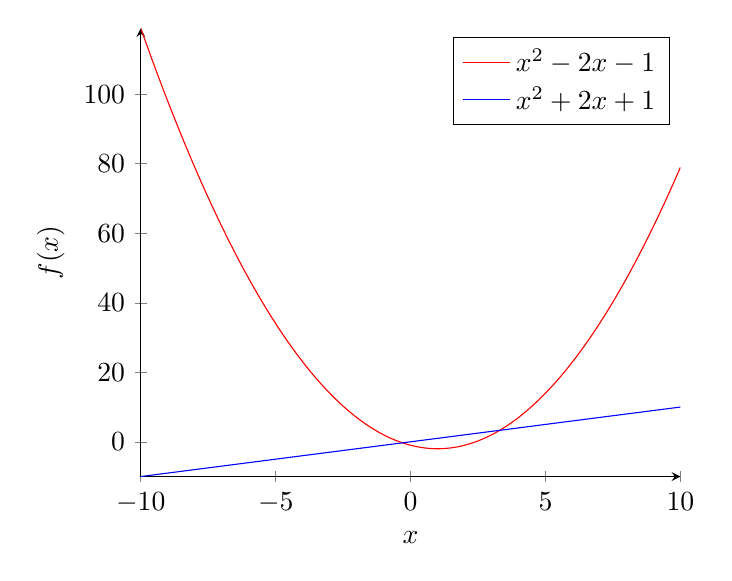
\begin{tikzpicture}
\begin{axis}[
    axis lines = left,
    xlabel = $x$,
    ylabel = {$f(x)$},
]
%Below the red parabola is defined
\addplot [
    domain=-10:10,
    samples=100,
    color=red,
]
{x^2 - 2*x - 1};
\addlegendentry{$x^2 - 2x - 1$}
%Here the blue parabloa is defined
\addplot [
    domain=-10:10,
    samples=100,
    color=blue,
    ]
    {x};
\addlegendentry{$x^2 + 2x + 1$}


\end{axis}
\end{tikzpicture}
\end{center}

The idea is simple, given a prey $P$, we would like to draw the curve of the predator $PR$ where the predator is pursuing $P$ such that $PR$ is always directly running at $P$.
However, the ratio of their velocities always remains a constant $K$.

\begin{enumerate}

\qitem Provided the velocities $\vec{V}_{P}$ and $\vec{V}_{PR}$, the positions $P$ and $PR$, write out a system of vector differential equations that describes this relationship in any number of dimensions.

\sol{
We can model this scenario with the following set of equations.
First, we know that the ratio of their velocities are always constant.
We also know that because $PR$ runs directly at $P$, the unit vector described by $P - PR$ is the same as the unit vector describing the velocity of $PR$.
This is because velocity is just magnitude and direction.
Thus, we get the following:

\begin{gather*}
K = \frac{\left\lVert\vec{V}_{PR}\right\rVert}{\left\lVert\vec{V}_{P}\right\rVert} \\
\frac{\vec{V}_{PR}}{\left\lVert \vec{V}_{PR} \right\rVert} = \frac{P - PR}{\left\lVert P - PR \right\rVert}
\end{gather*}


Substituting one into the other, we the following:

\begin{align*}
\vec{V}_{PR} = K \left\lVert \vec{V}_{p} \right\rVert \frac{P - PR}{\left\lVert P - PR \right\rVert}
\end{align*}

}



\end{enumerate}

\end{qunlist}

\end{document}
